

\frame{\frametitle{ A little about myself}
\begin{itemize}
\item 1985ish Life started with BASIC on a  commodore 
\item 1993 graduated  Computer Science Degree and Masters University College Cork, Ireland 
\item 1993 - 1997 Spacecraft Control Systems (C++) in ESA Mission Operations Centre Darmstadt Germany
\item 1997 - 2001 Hipparcos, Integral, Planck, Gaia, Bepi-Sax  (C,Java,Oracle, HTM, HEALPix) in ESA Technology Research Centre Noordwijk Netherlands
\item 2001-2003 Commercial programming - some Astronomy (Java) 
\item 2003-2005 The Johns Hopkins, SDSS and National Virtual Observatory (C,C\#,Java,Sqlserver)
\item 2005-2014 Gaia Astrometric Solution and Science Operations (Java, Oracle, Intersystems Cache) 
\item 2012  PhD in Physics on Implementing the Gaia Astrometric Solution,  Barcelona University
\item 2014-2017 All ESA Science Ground Segments in Development
\end{itemize}
}

\frame{\frametitle{Induction to astronomy : HIP Catalogue}
1997/98 Hipparcos Java Tools - learning Astrometry
\url{http://www.cosmos.esa.int/web/hipparcos/java-tools}
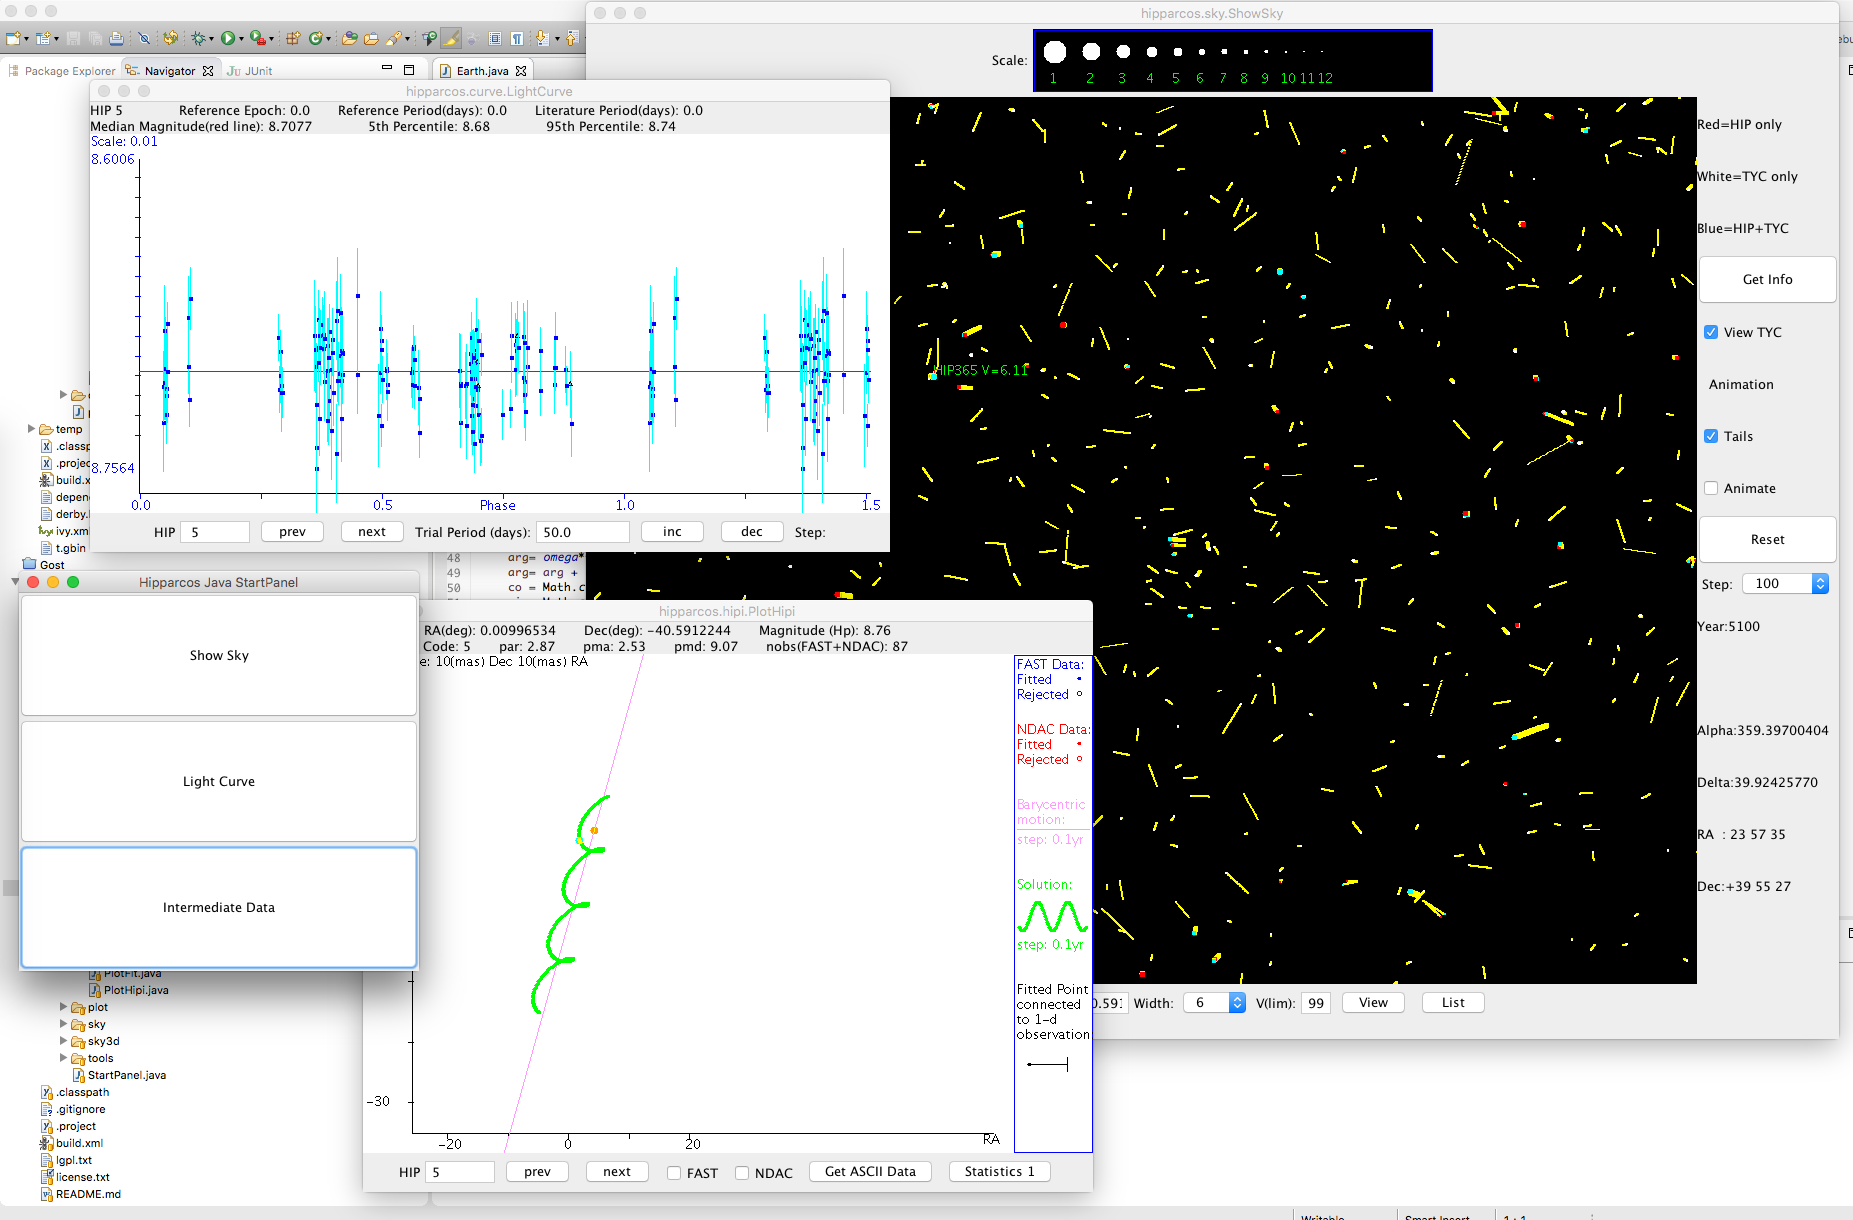
\includegraphics[width=\textwidth]{hipjt}
}

\frame{\frametitle{In the USA .. }
\vspace{5pt}
\begin{columns}[c]
\column{0.6\textwidth}
\vspace{4pt}
Quality tools for GSC2 (Java) $\rightarrow$\\
\vspace{8pt}
CasJobs (C\#)\citep{conf:casjobs}
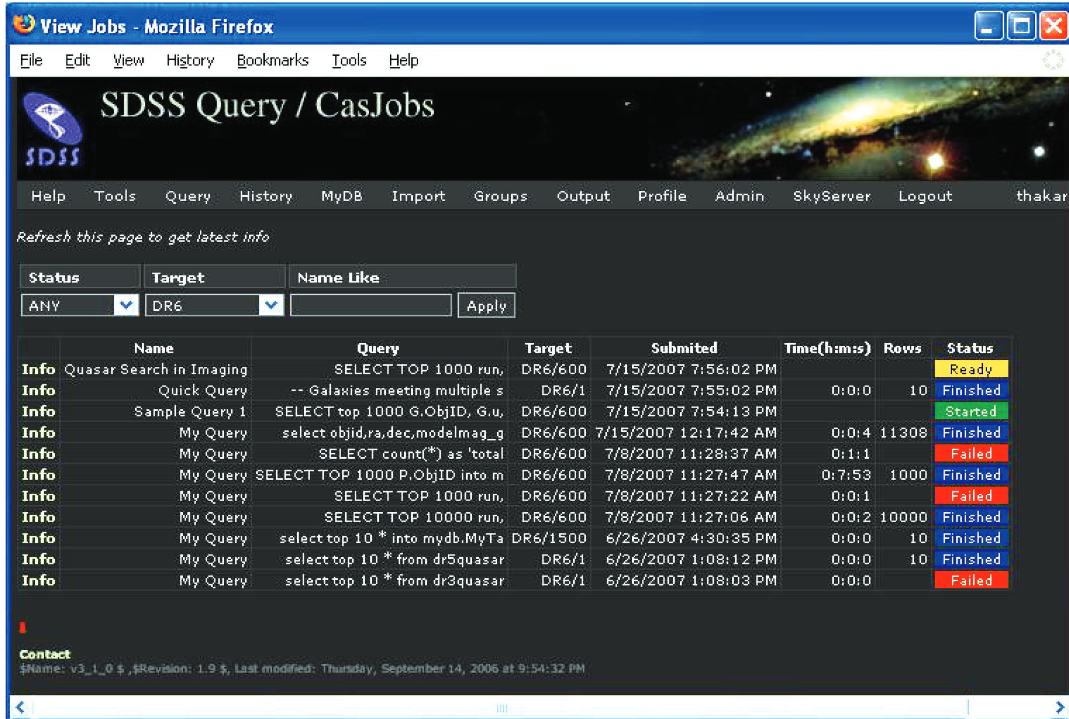
\includegraphics[width=\textwidth]{casjobs}
\column{0.4\textwidth}
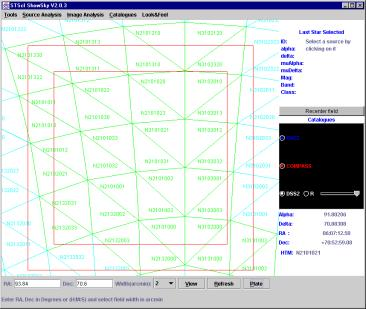
\includegraphics[width=\textwidth]{sshtm}
\vspace{-1cm}
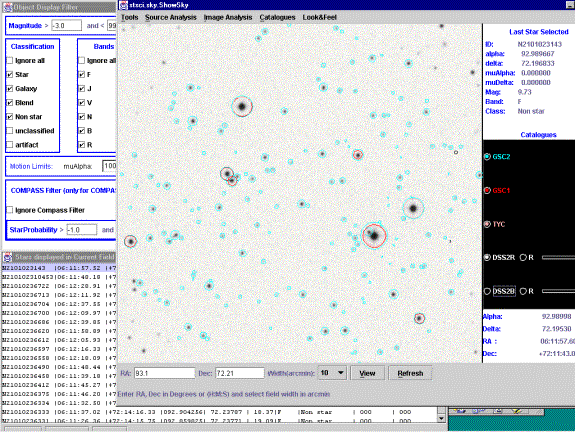
\includegraphics[width=\textwidth]{showsky}
\end{columns}
}


\frame{\frametitle{European Space Astronomy Centre }
\begin{columns}[c]
\column{0.4\textwidth}

\includegraphics[width=0.9\textwidth]{exm}\\

\includegraphics[width=0.45\textwidth]{bepiclogo}
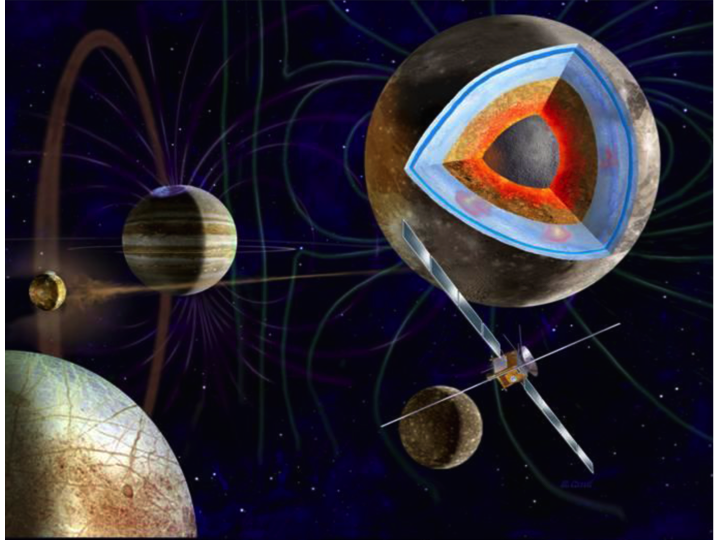
\includegraphics[width=0.45\textwidth]{juice}\\
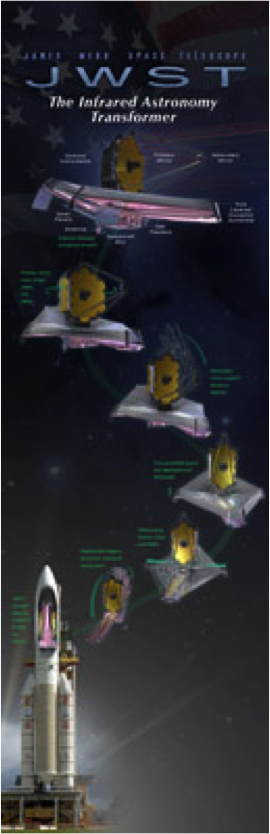
\includegraphics[width=0.45\textwidth]{jwst}\\
\vspace{-6cm}
\hspace{2.2cm}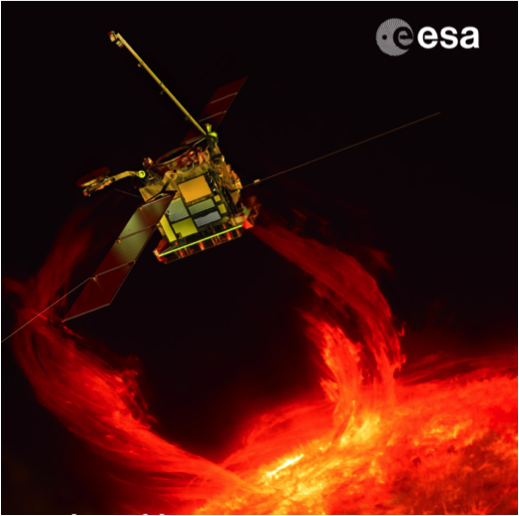
\includegraphics[width=0.45\textwidth]{solo}\\
\hspace{2.2cm}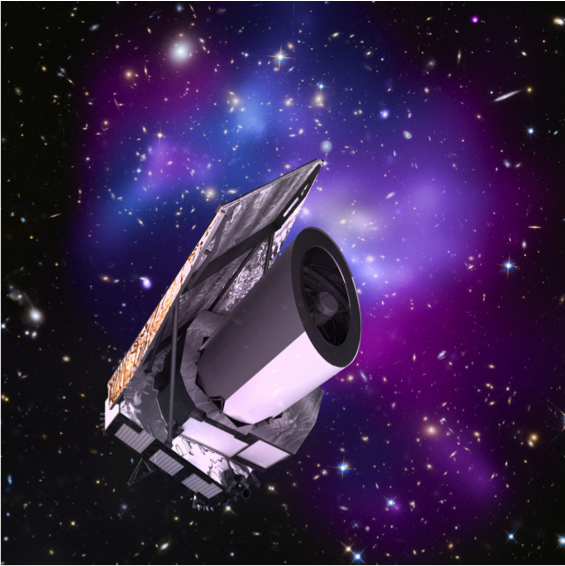
\includegraphics[width=0.45\textwidth]{euclid}

\column{0.6\textwidth}
\begin{itemize}
\item ESAC Located near Madrid, Spain.
\item Home of the Science Operations Department  containing  Operations Development Division.
\item Develop Science Operations Systems:
\begin{itemize}
\item People, Procedures and Software.
\item Interactions MOC and scientific communities.
\item Quite a bit of software - diverse - mainly Java but FORTRAN, C, C++, Python ..
\item Prepare for planning, simulations, instrument performance, commanding.
\item Hand over system to operations division after commissioning.

\end{itemize}
\end{itemize}
\end{columns}
}



